\chapter{Architectural Decision Records}
    \section{Definition, Role and Use}
        An emerging way to capture architectural design decisions (ADDs) and prevent knowledge vaporization are architectural decision records(ADRs).\allowbreak ADRs are lightweight text artifacts that capture the rationale behind ADDs by outlining some of the basic structure of such decisions\cite{MarkdownADRs}. Their simple nature allows them to be stored alongside other software artifacts such as source code in software repositories, internal company wikis and regular documentation \cite{DOCUMENTING_ARCHITECTURE_DECISIONS}. They can also be put under version control systems like Git in order to preserve their modification history as the requirements of the system in question change but they are mostly viewed as an append-only log \cite{microsoftArchitectureDecision} and thus, they are immutable. This means that if the need to revisit an existing architecture arises, there is a need to create an entirely new ADR and not modify any existing ones. Version control of ADRs also enables the collaboration of multiple people on the same document, facilitating group decision making, along with the option for reviews of AD by the means of ``pull requests'' which are valuable feature but are absent in many AKM tools \cite{compare_study_adr_tools}. In a given repository, ADRs are usually stored in a folder path similar to \textbf{doc/adr} or \textbf{doc/arch} \cite{github_page_adrs}. Their proposed naming convention\footnote{https://github.com/joelparkerhenderson/architecture-decision-record?tab=readme-ov-file\#file-name-conventions-for-adrs} is that they should first start with the string ``adr'' followed by a number starting from 001 that is incremented with each new record. These are followed by a brief title of the decision in lowercase. Finally, all naming sections are separated with hyphens to promote readability. For example, the name of an ADR that refers to the use the OpenAI API for a new web application can look like \textbf{``adr-001-use-openai-api.md''}.
        
        ADRs are template-based documents which come in many styles and formats, some of which are presented in the next section. ADRs are employed by prominent companies in the field of software engineering that produce engineering blogs read by thousands of practitioners such as Microsoft and Spotify \cite{Spotify_ADRS, microsoftArchitectureDecision}. 
        
        ADRs provide a practical solution to some ever-present problems of software architects. Firstly, they combat the documentation fatigue that architects experience when making decisions by having a minimalist format and being easy to store and manage. In one of the biggest software architect surveys \cite{architect_survey2} ``none of the interviewees reported using knowledge or decision management tools to manage project-related architectural knowledge. Instead, they mentioned text documents (64\%), source code (60\%), wikis (56\%), project diaries and meeting minutes (40percent), and issue management systems (20\%)''. So ADRs, by being text-based and close to source code, are already aligned with the most popular architecture documentation practices amongst practitioners. Because of this, they also minimize friction and effort for software architects, thus proving to be a viable alternative to consider for many practitioners in the field. A collection of ADRs in a project or organization, constitute an architecture decision log (ADL) that acts as a source of truth for ADDs.
        
    \section{Types of ADRs and Tool Support}
        Numerous types and templates of ADRs have been proposed, each one catering to a specific use case and making use of different patterns observed in architectural decision making. The most common and versatile format, present in the majority of software repositories that contain ADRs is the template proposed by Michael Nygard (NY) \cite{Github_study_ADRs}. Michael Nygard proposes a minimalist markdown document consisting of four distinct sections.
        \begin{enumerate}
        \item The \textbf{Status} of the AD, which can be anything from ``proposed, accepted, rejected, deprecated, or superseded'' that indicates the stage the decision is in.
        \item The \textbf{Context} of the decision that provides an overview of the problem and the motivation behind the efforts of trying to find a solution to this problem. Some best practices for this section include adding organization-specific context and business priorities, considerations based on social and technical skills of the teams that work within the organization and relevant pros and cons.
        \item The \textbf{Decision} proposed to solve the issue. This can be a concrete decision such as the use of a technology or something less specific such as the decision to adhere to a certain standard.
        \item The \textbf{Consequences} associated with the decision. This refers to consequences not only on the components of the system structure that are being affected by the AD but also to outcomes and outputs about the system as a whole and all of the dependencies that it may have.
        \end{enumerate}. 
        If any additional requirements are imposed as a direct consequence of the decision, this section should also link to the subsequent ADRs created.
        An example of this format can be seen in figure \ref{fig:ADR_Example_MN}. The document also contains references to other past ADRs in the ``Context'' section, indicating the ease of dependency management between ADs. From references like these a dependency graph can be constructed to not only visualize the various ADs along the projects life but also identify potential requirement conflicts or circular dependencies. All of these sections are also in line with the architectural decision making process by making use of some important considerations an architect makes as mentioned in the previous chapter. 

        \begin{figure}
            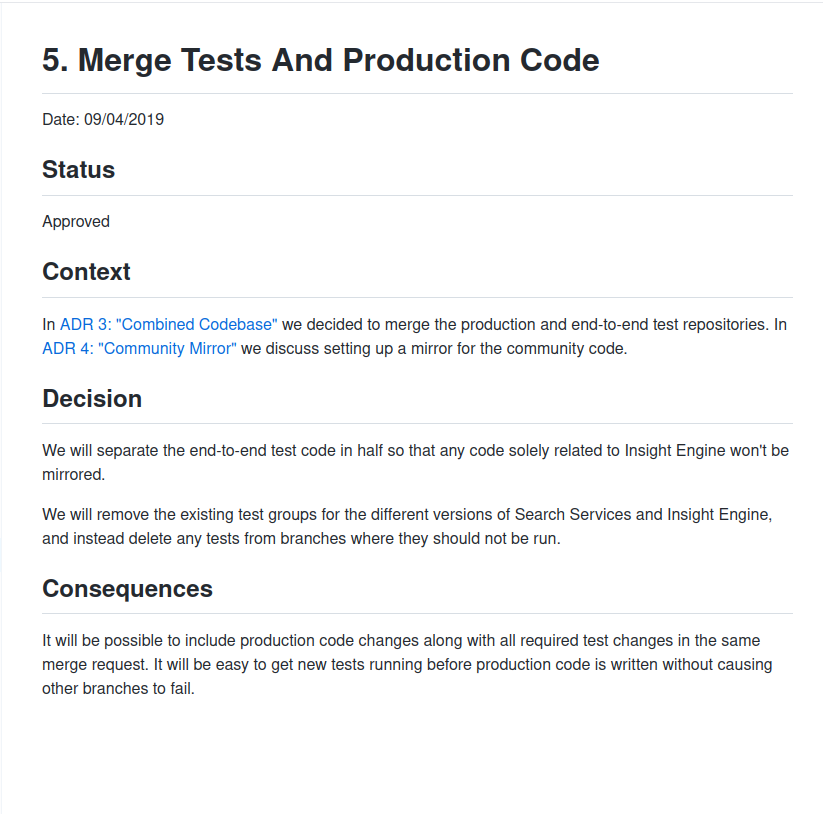
\includegraphics[scale=0.5]{figures/ADR_Example.png}
            \caption{ADR Example used by an open source project using the template format proposed by Michael Nygard}
            \label{fig:ADR_Example_MN}
        \end{figure}

        Numerous other ADR templates have been proposed. Tyree and Akerman's (\textbf{TA}) Template, is one of the first templates proposed that enriches the document with sections such as ``Constraints'', that reduce the solution space, ``Grouping'', that states how the new component will tie in to the existing system structure, and an ``Argument'' section that rationalizes the decision. The markdown ADR (MADR) (\textbf{MD}) template\cite{MarkdownADRs} on the other hand describes the problem as a ``User Story'', that resembles a ticketing system reference and the decision is motivated by ``Decision Drivers''. It can also outline the decision alternatives in detail in each separate section. The Alexandrian template pattern (AP) is also a simple document containing solely two sections, an ``Introduction'', that defines the problem in a summary, the decision made and its results, and a ``Specifics'' section that gives more context on both the solution, the problem (as a story of the current state of things and the quality of the options considered. The Business Case ADR (BC) template views the document from a perspective of a business analyst that oversees architectural decisions. It focuses on evaluation criteria, candidate solutions, and associated costs. When it comes to sections, it includes a top-level overview of the problem that eventually leads to a recommendation on how to solve it. For each solution candidate, it provides a detailed analysis covering how the candidates were discovered, research methods, criteria fulfillment, cost analysis, SWOT analysis, and internal and external opinions. Lastly, the Planguage (PL) template is more quality assurance oriented. It uses a special informal, but structured, keyword-driven
        planning language that can be used to create rich specification of requirements solely using keywords such as ``Tag'', ``Gist'', ``Requirement'', ``Rationale'', ``Priority'', ``Stakeholders'',  ``Author'', ``Revision'', ``Date'', ``Assumptions'' in a format that is not separated by sections but instead resembles a database entry that can be indexed efficiently and reducing ambiguity. A detailed comparison of each template along with some of the most common sections mentioned in them can be seen in the table in \ref{table:adr_template_comparison}. Each ``+'' symbol signifies the presence of the section title of the far left column whereas each ``-'' signifies its absence in that specific format.  
    
        \newpage
        \begin{longtable}{|m{5cm}|c|c|c|c|c|c|}
    \hline
    % Nygard , Tyree \& Akerman , Alexandrian Pattern, Business Case, MADR , Planguage
    \textbf{Feature} & \textbf{NY} & \textbf{TA} & \textbf{AP} & \textbf{BC} & \textbf{MD} & \textbf{PL} \\
    \hline
    \textbf{Title} & + & + & - & + & + & + \\
    \hline
    \textbf{Status} & + & + & - & + & + & + \\
    \hline
    \textbf{Context/Background} & + & - & + & + & + & + \\
    \hline
    \textbf{Problem/Issue} & + & + & + & + & + & + \\
    \hline
    \textbf{Forces/Decision Drivers} & - & - & + & - & + & - \\
    \hline
    \textbf{Decision} & + & + & + & + & + & + \\
    \hline
    \textbf{Options} & - & - & - & + & + & + \\
    \hline
    \textbf{Solution} & + & + & + & + & + & + \\
    \hline
    \textbf{Consequences
    /Implications} & + & + & + & + & + & + \\
    \hline
    \textbf{Motivation/
    Rationale} & - & + & - & - & + & + \\
    \hline
    \textbf{Assumptions} & - & + & - & - & - & - \\
    \hline
    \textbf{Related Decisions} & - & + & - & - & - & - \\
    \hline
    \textbf{Stakeholders} & - & - & - & - & - & + \\
    \hline
    \textbf{Pros and Cons} & - & - & - & - & + & - \\
    \hline
    \caption{Comparison of ADR Templates}
    \label{table:adr_template_comparison}
\end{longtable}

        Tool support for creating and managing ADRs is currently limited to few but powerful options. One of the most popular alternatives is ``ADR Tools''\footnote{https://github.com/npryce/adr-tools}. It is a command-line utility that is close to the development lifecycle and helps manage ADRs by providing commands to create, maintain, and visualize these records in a project. It has beed implemented in many programming languages with slight variations, showcasing its popularity. Other tools such as ``Loqbooq''\footnote{https://loqbooq.app/} and ``adr-manager''\footnote{adr-manager} are web applications focusing on simplicity when managing ADRs, while other libraries such as ``Embedded Architectural Decision Records''\footnote{https://github.com/adr/e-adr\#embedded-architectural-decision-records} for Java and ``architectural-decision''\footnote{https://github.com/cspray/architectural-decision} for PHP provide the option to embed ADRs inside functional code. The later can also be a viable option for organizations that prefer only writing code comments for documenting all aspects related to system code.

    \newpage
    \section{ADRs in Practice}
        % Spotify + overview of process if needed
        ADRs have been used in practice and its use endorsed by prominent organizations. One example is Spotify \cite{Spotify_ADRS} that reports benefits such as ease of onboarding of new engineers, since new hires are able to get up to speed with code and system principles faster instead of discovering them as they navigate the challenges of their work. This proves that since ADRs also constitute a piece of AK, they can enhance knowledge sharing across stakeholders and geographically distributed teams (such as those in Spotify) \cite{AK_management} by removing barriers to knowledge management systems. They also report that ADRs enable more efficient ownership handover in organizations that do frequent internal restructuring of departments as they lower the friction of information transferring and allow for a seamless system ownership transition to new teams. Finally they facilitate alignment between different parts of an organization by providing a single source of truth for all architecture related decisions.

        % Redhat
        ADRs are also encouraged by Red Hat\footnote{https://www.redhat.com/architect/architecture-decision-records} especially paired with the Open Decision Framework\footnote{https://opensource.com/open-organization/resources/open-decision-framework} which is a set of best practices developed by Red Hat for making transparent, inclusive decisions in organizations that adhere to open source principles, focusing on collaboration, diverse perspectives, and clear communication. They state that when the architectural decision affects multiple stakeholders, it can be integrated in an ADR feedback loop facilitated by a pull request, focusing on open source principles.  

        % Amazon + overview of process if needed
        Amazon and its cloud service, Amazon Web Services (AWS) also highlight the need of ADRs as key architectural documentation\footnote{https://docs.aws.amazon.com/prescriptive-guidance/latest/architectural-decision-records/} as it ``streamlines technical decision-making'', by providing a structured process for documenting, justifying, and communicating architectural decisions. They explicitly mention architectural decision repositories as a means of storing such knowledge. Inside AWS, ADRs help align team members with the strategic direction a system may be taking, set general project directions and guidelines, and avoid common decision-making pitfalls by capturing the context, rationale and solutions behind past experiences. Furthermore, they state that ADRs can reduce development time, improve documentation, and enhance the handover process for future teams, ensuring that critical information is preserved and is indexed and accessible. 